\documentclass{article}

\usepackage{booktabs}
\usepackage{tabularx}
\usepackage{hyperref}
\usepackage[a4paper, margin=0.75in]{geometry}
\usepackage{graphicx}
\usepackage{subcaption}
\usepackage{float}

\hypersetup{
    colorlinks=true,       % false: boxed links; true: colored links
    linkcolor=red,          % color of internal links (change box color with linkbordercolor)
    citecolor=green,        % color of links to bibliography
    filecolor=magenta,      % color of file links
    urlcolor=cyan           % color of external links
}

\title{Hazard Analysis\\\progname}

\author{\authname}

\date{}

%% Comments

\usepackage{color}

\newif\ifcomments\commentstrue %displays comments
%\newif\ifcomments\commentsfalse %so that comments do not display

\ifcomments
\newcommand{\authornote}[3]{\textcolor{#1}{[#3 ---#2]}}
\newcommand{\todo}[1]{\textcolor{red}{[TODO: #1]}}
\else
\newcommand{\authornote}[3]{}
\newcommand{\todo}[1]{}
\fi

\newcommand{\wss}[1]{\authornote{magenta}{SS}{#1}} 
\newcommand{\plt}[1]{\authornote{cyan}{TPLT}{#1}} %For explanation of the template
\newcommand{\an}[1]{\authornote{cyan}{Author}{#1}}

%% Common Parts

\newcommand{\progname}{ProgName} % PUT YOUR PROGRAM NAME HERE
\newcommand{\authname}{Team \#, Team Name
\\ Student 1 name
\\ Student 2 name
\\ Student 3 name
\\ Student 4 name} % AUTHOR NAMES                  

\usepackage{hyperref}
    \hypersetup{colorlinks=true, linkcolor=blue, citecolor=blue, filecolor=blue,
                urlcolor=blue, unicode=false}
    \urlstyle{same}
                                


\begin{document}

\maketitle
\thispagestyle{empty}

~\newpage

\pagenumbering{roman}

\begin{table}[hp]
\caption{Revision History} \label{TblRevisionHistory}
\begin{tabularx}{\textwidth}{c l X l}
\toprule
\textbf{\#} & \textbf{Author(s)} & \textbf{Description of Changes} & \textbf{Date}\\
\midrule
0 & All & Created first draft of the document & 2025-10-10\\
\bottomrule
\end{tabularx}
\end{table}

~\newpage

\tableofcontents

~\newpage

\pagenumbering{arabic}


\section{Introduction}

This document outlines the hazard analysis of the \textbf{Large Event Management System (LEMS)} for the McMaster
Engineering Society (MES). The LEMS is a centralized platform designed to streamline event workflows such as
 \textbf{ticket sales, registrations, waivers, payments, bus/table sign-ups, notifications, and event check-ins}.'
\newline

\noindent
For this deliverable, the analysis will specifically focus on the features within the scope of \textbf{Project B} which include:

\begin{itemize}
    \item Payment System
    \item Role-Centric/Feature-Based Access Control (RBAC/FBAC)
    \item Bus Sign-Ups
    \item RSVP Sign-Ups
    \item Table Sign-Ups
\end{itemize}

\noindent
Hazards in this system refer to conditions or failures that may lead to financial loss, security/privacy breaches,
accessibility failures, or reputational damage for MES and McMaster University. While the system does not directly
involve hardware or pose risks of physical harm, software risks are significant. These include data loss, payment
errors, registration corruption, check-in failures, and unauthorized access to sensitive information.
\newline

\noindent
The purpose of this hazard analysis is to:

\begin{itemize}
    \item Identify risks associated with the Payment, Access Control, and Signup modules.
    \item Define their potential impacts on users, organizers, and the MES organization.
    \item Introduce mitigation strategies by specifying safety and security requirements that
     will guide system design and implementation.
\end{itemize}

\noindent
By proactively addressing these hazards, this analysis ensures the system will be reliable, secure, accessible, and trustworthy for both organizers and attendees.

\section{Scope and Purpose of Hazard Analysis}


The purpose of this hazard analysis is to identify and evaluate potential hazards that could arise during 
the development and operation of the Large Event Management System (LEMS). Since LEMS is a 
software-based platform that supports event registration, ticketing, payments, and participant 
management, hazards are primarily related to data integrity, system availability, security, and user 
interactions. By analyzing these risks early, the project team can define mitigation strategies, 
incorporate safety and security requirements into the design, and reduce the likelihood of 
organizational or reputational harm.

\par
\vspace{1em}

The scope of this analysis covers all major components of LEMS, including the backend services, 
web and mobile applications, and the database. It considers hazards introduced by user error, software 
defects, integration failures across modules, and security vulnerabilities. Hazards that fall outside the 
team’s control, such as third-party cloud hosting failures or issues with external payment providers 
(e.g., Stripe), are acknowledged but not analyzed in detail.

\par
\vspace{1em}

The goals of this hazard analysis are:
\begin{itemize}
  \item To proactively identify risks related to security, data integrity, privacy, and availability in LEMS.
  \item To evaluate the potential consequences of failures, such as data loss, financial errors, or 
        unauthorized access to sensitive information.
  \item To define mitigations or controls that reduce these risks to acceptable levels.
  \item To guide architectural and design decisions and support the definition of non-functional 
        requirements such as reliability, security, and maintainability.
\end{itemize}

This hazard analysis will be refined as the project design evolves, ensuring that new risks are 
addressed as they emerge. It is part of the broader quality assurance process and ensures that LEMS 
meets the standards of safety, security, and reliability expected by the McMaster Engineering Society.

\section{System Boundaries and Components}

The MacSync platform system that the hazard analysis will be conducted on consists of:
\begin{enumerate}
    \item The application that is both web and mobile based, which includes the front-end and back-end made up of the following major components:
    \begin{itemize}
        \item Dashboards (User and Admin)
        \item Payment System
        \item Authentication (Role/Feature Based Access Control)
        \item RSVP Sign-Ups
        \item Bus Sign-Ups
        \item Table Sign-Ups
    \end{itemize}
    \item The PostgreSQL database where all user, admin, event and transaction data will be stored.
    \item The payment module that interfaces with external payment gateways to process ticket payments and refunds.
    \item The notification service that sends automated emails and notifications to users for event details and payment receipts.
\end{enumerate}

The system boundary in the case of the MacSync platform includes components necessary to support event operations for the MES, which includes the entire application, both web and mobile based, along with their subcomponents, the database, payment gateway and notification service. The payment and notification services are controlled by external providers. The payment is controlled by Stripe and the notification service is controlled by Microsoft. However, they remain critical to the function of the system and the overall operation of the platform and thus fall within the system boundary.

\section{Critical Assumptions}

The following assumptions have been identified as critical to the safe and reliable operation of the MacSync platform.

\begin{itemize}
    \item \textbf{Reliable Internet Access:} It is assumed that both attendees and organizers will have access to stable internet connections during registration, payment, and check-in. While temporary connectivity loss may occur, the system must handle these cases gracefully.
    
    \item \textbf{Third-Party Service Availability:} The platform depends on external services such as payment processors (e.g., Stripe, PayPal) and hosting infrastructure. It is assumed these services provide high availability, but the system will still account for outages or delays to prevent complete operational failure.
    
    \item \textbf{Device Compatibility:} It is assumed that attendees will primarily use modern smartphones and organizers will have access to laptops or mobile devices capable of running the dashboard. Reliance on outdated devices or unsupported browsers must be minimized through compatibility testing.
    
    \item \textbf{User Data Accuracy:} The system assumes that users provide correct information (e.g., dietary restrictions, accessibility needs, payment details). However, hazards tied to incorrect or incomplete inputs will be addressed by validation checks.
    
    \item \textbf{Organizational Oversight:} It is assumed that event organizers will actively monitor the system for anomalies (e.g., payment disputes, capacity errors, failed notifications). This system will assist and automate many of the tasks and centralize information, but human oversight is still necessary to manage unexpected situations.
    
    \item \textbf{Security Measures:} It is assumed that standard security practices (encrypted storage, secure authentication, and role-based access control) will be implemented and maintained. Failure to enforce these could expose sensitive student data or enable fraudulent event access.
\end{itemize}


\section{Failure Mode and Effect Analysis}

The Failure Mode \& Effect Analysis (FMEA) is the tool chosen to identify possible hazards within the system. Identifying these hazards will allow the creation of strategies to mitigate them.

\subsection{Hazards Out of Scope}
The following hazards fall outside the control of the dev team however, still have a critical impact on system operations:
\begin{enumerate}
    \item The users mobile device
    \item Hosting provider availability
    \item External payment gateway provider availability
    \item Any External API's hosted by third-party providers (ie. Calendars, Database, OAuth)
\end{enumerate}
These dependecies are all hosted by third party services and therefore the development team cannot control the downtime or availability of them. However, an attempt will be made to mitigate these hazards as much as possible in the case they occur.

\subsection{Failure Modes \& Effects Analysis Table}

\begin{figure}[H]
\begin{subfigure}{\textwidth}
    \centering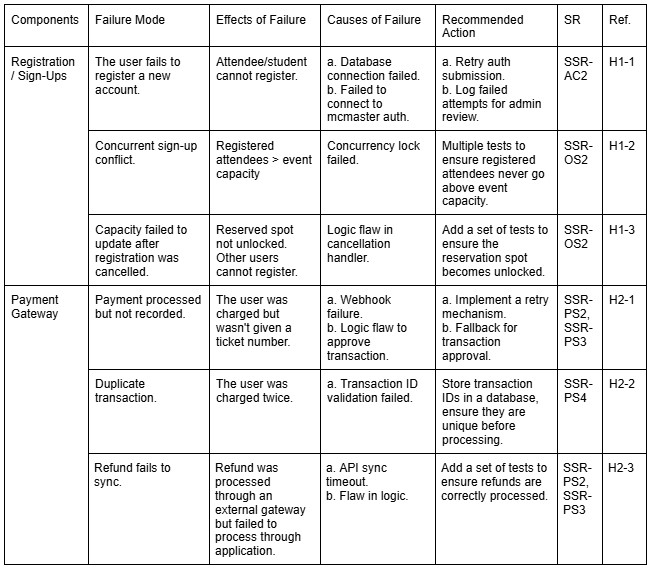
\includegraphics[width=\textwidth]{part1-register_payment.jpg} 
    \caption{FMEA Table Part 1}
\end{subfigure}

\begin{subfigure}{\textwidth}
    \centering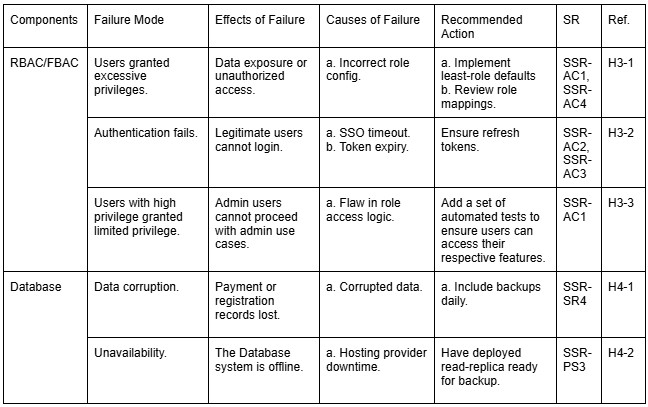
\includegraphics[width=\textwidth]{part2-rbac_db.jpg} 
    \caption{FMEA Table Part 1}
\end{subfigure}

\end{figure}

\section{Safety and Security Requirements}

\subsection{Data Security Requirements}
\begin{itemize}
    \item \textbf{SSR-DS1 (Encryption in Transit):} The system shall use TLS 1.2 or higher to encrypt all network communications between client applications, servers, and third-party APIs.
    \item \textbf{SSR-DS2 (Encryption at Rest):} The system shall encrypt sensitive stored data (user profiles, accessibility needs, dietary restrictions, waiver records) using AES-256.
    \item \textbf{SSR-DS3 (Privacy Compliance):} The system shall comply with PIPEDA and relevant McMaster University policies regarding data collection, storage, and retention.
    \item \textbf{SSR-DS4 (Data Minimization):} The system shall only store the minimum personal data necessary for event operations (e.g., no raw payment card details).
\end{itemize}

\subsection{Payment Security Requirements}
\begin{itemize}
    \item \textbf{SSR-PS1 (Third-Party Gateways):} All financial transactions shall be processed exclusively through secure payment providers (Stripe, Square, or PayPal). The system shall not store or transmit raw credit card details.
    \item \textbf{SSR-PS2 (Transaction Confirmation):} The system shall generate a unique transaction confirmation code for every payment, retrievable by both the attendee and the organizer.
    \item \textbf{SSR-PS3 (Audit Logging):} All financial operations (payments, refunds, chargebacks) shall be logged in an immutable audit trail accessible only to authorized financial officers.
    \item \textbf{SSR-PS4 (Duplicate Protection):} The system shall prevent duplicate payments by checking for transaction IDs before ticket issuance.
\end{itemize}

\subsection{Access Control Requirements}
\begin{itemize}
    \item \textbf{SSR-AC1 (Role-Based Access Control):} The system shall enforce RBAC/FBAC to ensure that each organizer only has access to the features necessary for their role.
    \item \textbf{SSR-AC2 (Authentication):} The system shall integrate with McMaster University's Single Sign-On (SSO) to authenticate student attendees and organizers.
    \item \textbf{SSR-AC3 (Session Management):} The system shall automatically expire inactive sessions after 15 minutes of inactivity for admin accounts and 60 minutes for attendee accounts.
    \item \textbf{SSR-AC4 (Privilege Escalation Protection):} The system shall log and alert MES executives of any attempts at unauthorized access or privilege escalation.
\end{itemize}

\subsection{System Reliability \& Availability Requirements}
\begin{itemize}
    \item \textbf{SSR-SR1 (Uptime):} The system shall maintain at least 98\% uptime during active registration and event check-in periods.
    \item \textbf{SSR-SR2 (Offline Check-in):} The system shall support offline QR code validation to allow event entry if internet connectivity is unavailable.
    \item \textbf{SSR-SR3 (Notification Redundancy):} All time-sensitive notifications (registration confirmations, event reminders) shall include retry mechanisms to ensure delivery.
    \item \textbf{SSR-SR4 (Backup \& Recovery):} The system shall automatically back up all event and registration data daily and enable recovery within 24 hours of data loss.
\end{itemize}

\subsection{Operational Safety Requirements}
\begin{itemize}
    \item \textbf{SSR-OS1 (Waiver Enforcement):} The system shall not allow final ticket confirmation until the attendee has digitally signed the required waiver.
    \item \textbf{SSR-OS2 (Capacity Validation):} The system shall enforce real-time capacity limits for bus sign-ups, table sign-ups, and RSVP sign-ups to prevent overbooking.
    \item \textbf{SSR-OS3 (Organizer Accountability):} All organizer actions (e.g., modifying capacities, issuing refunds, editing registrations) shall be logged with a timestamp and user identifier.
    \item \textbf{SSR-OS4 (Fail-Safe Defaults):} In the event of a system error, the system shall default to denying access to sensitive data until the error is resolved.
\end{itemize}


\section{Roadmap}

The implementation of safety and security requirements for the Large Event Management System will occur in stages aligned with the capstone development timeline. Due to the limited duration of the project, the focus will be on ensuring that all critical safety mechanisms which are directly affecting system reliability, security, and data integrity are implemented and validated within the current term. Remaining requirements will be planned for integration by the McMaster Engineering Society (MES) technical team during future development cycles.

\subsection*{Implemented During Capstone Timeline}
The following requirements will be implemented during the capstone term as part of the system’s core functionality:
\begin{itemize}
    \item \textbf{Data Security:} TLS encryption for data in transit (SSR-DS1) and AES encryption for sensitive data at rest (SSR-DS2).
    \item \textbf{Payment Security:} Secure integration with a third-party payment gateway (SSR-PS1), unique transaction confirmation codes (SSR-PS2), and duplicate transaction protection (SSR-PS4).
    \item \textbf{Access Control:} Role-Based Access Control (RBAC/FBAC) (SSR-AC1) and session management enforcement (SSR-AC3) for both web and mobile platforms.
    \item \textbf{System Reliability:} Real-time capacity validation for sign-ups (SSR-OS2), daily automated database backups (SSR-SR4), and fail-safe defaults on system errors (SSR-OS4).
    \item \textbf{Operational Safety:} Enforcement of waiver signing before ticket confirmation (SSR-OS1) and logging of organizer actions for traceability (SSR-OS3).
\end{itemize}

These requirements directly address the most immediate and impactful hazards identified in the analysis, particularly those related to data privacy, payment integrity, and access control. Their implementation within the capstone ensures a secure and stable baseline for core system operations.

\subsection*{Planned for Future Implementation}
The following requirements are identified as long-term improvements that extend beyond the capstone’s implementation schedule:
\begin{itemize}
    \item \textbf{Advanced Audit Logging:} Immutable financial and administrative audit trails for regulatory compliance (SSR-PS3, SSR-AC4).
    \item \textbf{High-Availability Features:} Automated failover, performance monitoring, and uptime guarantees beyond 98\% (SSR-SR1).
    \item \textbf{Offline Mode Enhancements:} Expanded offline functionality for attendee check-in and ticket validation (SSR-SR2).
    \item \textbf{Notification Redundancy:} Implementation of retry and multi-channel fallback mechanisms for time-sensitive notifications (SSR-SR3).
    \item \textbf{Single Sign-On (SSO) Integration:} Full integration with McMaster University’s SSO platform for authentication (SSR-AC2).
\end{itemize}

These requirements, while essential for long-term system robustness and maintainability, rely on extended infrastructure and resources provided by MES after the capstone handover. Their implementation will build on the security and reliability foundation established by the current development team.


\newpage{}

\section*{Appendix --- Reflection}

\wss{Not required for CAS 741}

The purpose of reflection questions is to give you a chance to assess your own
learning and that of your group as a whole, and to find ways to improve in the
future. Reflection is an important part of the learning process.  Reflection is
also an essential component of a successful software development process.  

Reflections are most interesting and useful when they're honest, even if the
stories they tell are imperfect. You will be marked based on your depth of
thought and analysis, and not based on the content of the reflections
themselves. Thus, for full marks we encourage you to answer openly and honestly
and to avoid simply writing ``what you think the evaluator wants to hear.''

Please answer the following questions.  Some questions can be answered on the
team level, but where appropriate, each team member should write their own
response:


\begin{enumerate}
    \item What went well while writing this deliverable? 
    
    \textbf{Ali:} What went really well was the work distribution. We had really even division of labour and it being done on a rotating method where each person gets one section was really helpful in giving members a good idea of what every section was about.

    \textbf{Abyan:} From an analytical standpoint, the team approached the Hazard Analysis with a strong balance of technical accuracy and practical reasoning. Each hazard was considered in the real context of the architecture, not just as an abstract risk. This allowed the team to identify safety concerns that were both realistic and relevant such as payment failures and data handling vulnerabilities. The document evolved through meaningful collaboration, with members bringing insights from different subsystems to ensure no component was overlooked. What went particularly well was the team’s ability to move beyond compliance-based thinking toward a proactive safety mindset.

    \textbf{Farhan:} Writing the Hazard Analysis went smoothly once the team established a clear understanding of the system’s structure and potential failure points. Our prior work on defining the system scope, roles, and data flow made it easier to identify where risks could emerge, specifically around payments, user data, and cross module data handling. The process encouraged the team to think more critically about system safety and resilience rather than just functionality.

    \textbf{Prerna:} Before beginning the deliverable we all organized a meeting to look over the required parts and what they might look like and we were able to divide them evenly among ourselves. Using the github issues and being able to assign each issue to each group member made it easy to see which ones we were all working on, completed, and reviewed, and also made aided in keeping us organized and on track. Since we divided it in a way where we would all each be working on every document each group member was always in the loop about what was happening in each document.

    \textbf{Mahad:} Working on the deliverable as a whole went really well especially with the streamlined workflow we had covering the division of work to the reviews. What also went well was the meeting organization and being able to stay on track for working on each task and having the opportunity to ask questions when needed.


    \item What pain points did you experience during this deliverable, and how
    did you resolve them?

    \textbf{Ali:} A pain point faced was trying to align the team on deadline dates especially with hectic schedules due to assignments and midterms being due around the deadline for this project. We resolved this issue by focusing our efforts in getting as much work done as possible and discussing issues during times we were guaranteed to be together and have free time such as during the lecture times and tutorial time.

    \textbf{Abyan:} One consistent challenge was distinguishing between true system hazards and general project risks. Early drafts blur the line between technical failures and broader management concerns such as scheduling or workload. This required several iterations to refine. Another pain point was ensuring that every identified hazard could be meaningfully connected to a mitigation or safety requirement avoiding speculative risks that could not be addressed within scope. The team resolved this by mapping each hazard directly to the system’s functional and safety requirements, which clarified responsibility and feasibility.

    \textbf{Farhan:} Collaborating across groups also helped surface hazards that individual members might not have initially considered, such as data integrity risks due to concurrent database writes or communication breakdowns between the mobile app and backend APIs. Overall, the deliverable strengthened our shared understanding of system dependencies and clarified design priorities for reliability and user trust.

    \textbf{Prerna:} Some pain points we experienced were that some parts we were working on relied heavily on another group members assigned parts, making it difficult to work on some of the parts until another group member was finished with them. Also if any edits needed to be made to a certain part, then the corresponding part which relied on it would also have to be changed. Trying to balance these deliverables with other course work was also difficult as some members had more coursework than others, adding some unforseen delays.

    \textbf{Mahad:} Some pain points we initially experienced was having to sometimes rely on other people's components to get work done which made it difficult to sometimes stay on top of work. However, we were easily able to resolve this through our meetings where we discussed priorities for each member and focused on getting the dependent work done first so team members were not roadblocked.


    \item Which of your listed risks had your team thought of before this
    deliverable, and which did you think of while doing this deliverable? For
    the latter ones (ones you thought of while doing the Hazard Analysis), how
    did they come about?

    Prior to doing the deliverable we had a strong idea on the technical risks related to the system. Specifically, we identified payment integration failures due to external API issues to be a big one very quickly because it is directly tied to a core functionality of the platform and one of the main components the team will be focused on developing. During the hazard analysis, we identified an additional risk which we did not fully consider before, which is associated with data security access within the role and feature based access control. This new risk we identified came about through breaking down the system into its main components and mapping system boundaries, wherein we realized how any failures or inaccuracies in this component could affect the overall reliability of the system as a whole.


    \item Other than the risk of physical harm (some projects may not have any
    appreciable risks of this form), list at least 2 other types of risk in
    software products. Why are they important to consider?
    
    Other than the risk of physical harm, two other major types of risks in software products include:
    \begin{enumerate}
        \item Data Privacy
        \begin{itemize}
            \item These risks mainly revolve around unauthorized access, data breaches and mishandling of sensitive users information. These risks are important to consider because of the severe consequences associated with them. For instance, mishandling of sensitive user information can lead to financial impact where there can be fines placed for not complying to regulations and there can be operational disruptions as well as reputational damage due to data breaches, which can lead to loss of customer trust and halt business operations.
        \end{itemize}
        \item Operational Reliability Risks
        \begin{itemize}
            \item These risks mainly revolve around the reliability of the system and its availability for users, specifically system failures, performance degradation and downtimes. These risks are important to consider because they can lead to customer usage disruptions and frustration. The result can be a loss in confidence in the dependability of the system as well as a loss of interest in the system, which can cause financial loss.
        \end{itemize}
    \end{enumerate}
    
\end{enumerate}
    
\end{document}